\subsection*{Runtime Efficiency}\label{subsec:runtime}
A consideration in a compiler is the performance or efficiency of its output. 
Rather than just translating the source code, translating to faster executable code is a subproblem in compiler optimisation.
Optimisation is however a nonspecific and absolute word, therefore in \gls{gamble} we will instead be referring to the problem as improving or increasing runtime efficiency.
Runtime efficiency entails considerations such as memory allocation, pipelining, parallelisation, which may have an impact on execution time.
To do an efficient and complete analysis of how to increase runtime efficiency, information of the situation in a given program is required.
This gives \gls{gamble} a disadvantage. 
\gls{gamble} abstracts its programmers from controlling where the code is performed and instead does so seamlessly.
Information about how e.g. a for-loop could be transformed into a kernel does not exist in \gls{gamble} which makes it difficult to do this.
The seamless use of the \acrshort{gpu} means that certain information is nonexistent and therefore all computations may not be candidates for improving its runtime efficiency, this is one of the trade-offs \gls{gamble} makes.
If \gls{gamble} were to require more information, e.g. whether or not something is paralleliseable or ask the programmer to determine what type of \acrshort{gpu} memory should be used for each variable; the simplicity and seamless use of the \acrshort{gpu} would be lost, and programming using Theano or directly using \gls{opencl} C might prove to be a better option.

As previously mentioned due to the object code being \gls{opencl} C certain considerations pertaining to instruction handling and register allocation etc. are not of interest for this compiler.
This is handled by using another compiler to compile the \gls{opencl} C code into machine code, see \myref{ssub:makefile}. 
To increase runtime efficiency the \gls{opencl} C code is the main target for improvements.

As \gls{gamble} is attempting to seamlessly use the \acrshort{gpu} to increase performance, knowing when the use of the \acrshort{gpu} will actually be beneficial is an important point in the code generation process. 
As mentioned to do this efficiently, the compiler would require more information about the computations in a \gls{gamble} program than can be read from the syntax of \gls{gamble}.
Therefore it is decided that it is better to be sure that a computation can benefit from the \acrshort{gpu}, rather than risking executing computations on the \acrshort{gpu} that will not benefit from its architecture.
As such only the operations that the project group knows have a possibility of benefiting from the parallel computational power of the \acrshort{gpu} will be executed on the \acrshort{gpu}.

%Knowing when to use GPU
Even though a computation can be parallelised, it does not necessarily mean it should be moved to the \acrshort{gpu}, as is evident in \myref{image:benchmark}.
This is an opportune moment for improving the runtime efficiency of the object code by using the \acrshort{gpu} only when it will be superior to the \acrshort{cpu} in regards to performance.
A possibility of doing so would be to analyse whether or not an instruction sequence both entail a sufficient amount of operations and that these are not sequentially dependent on each other.
Performing such an analysis increases compile time.
Because of the difficulty to discern not only if there will be an actual increase, but also if any custom functions created by a programmer are fit to be run on the \acrshort{gpu} this analysis is not part of the compiler.
Instead only vector and matrix operations already defined in the language, by having a special operator assigned to them, will be performed on the \acrshort{gpu}.

Kernel code uses explicit memory handling, and one must choose what memory space on the \acrshort{gpu} to allocate ones variables in as well as using the principle of locality.
This can provide a substantial (more than three times) faster runtime. \citep{ocl_lecture3}
\begin{figure}[h]
\centering	
 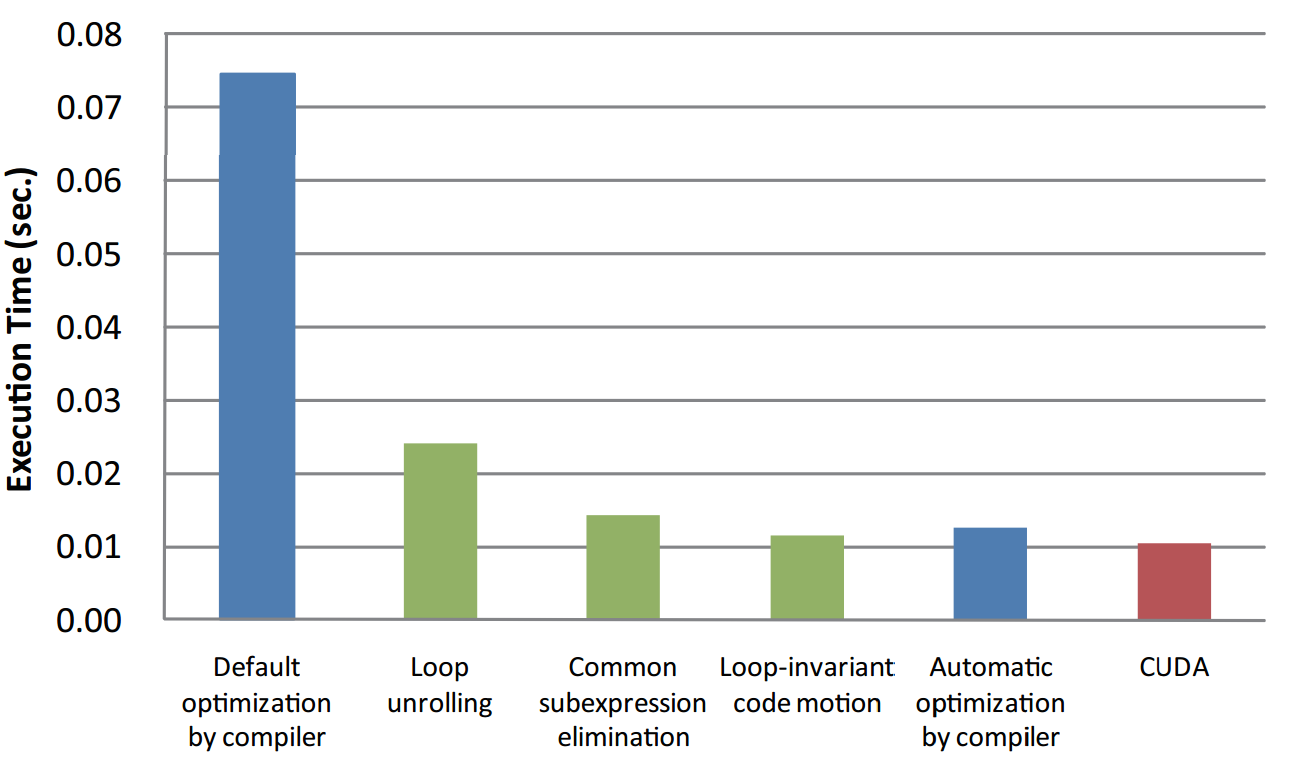
\includegraphics[width=1\textwidth]{figures/opencloptimisation.png} % trim=4.85cm 15cm 0.85cm 1cm
\caption{Execution speed of a matrix multiplication with different increases in runtime efficiency done. All bars except the \gls{cuda} bar represents \gls{opencl}. \todo[inline]{Det ville være TRIVIELT at forklare hvad disse optimeringer er og hvorfor programmet er hurtere på grund af det. Skal vi det? -- Troels -Let's do it homo!} \citep{CUDAOpenCLOptimisation}}\label{image:OpenCLOptCompare}
\vspace{-15pt}
\end{figure}
As seen on \myref{image:OpenCLOptCompare} some possible methods of increasing runtime efficiency includes loop unrolling, common sub-expression elimination and loop-invariant code motion. 
Loop unrolling is a technique that attempts to reduce, or if possible completely eliminate, instructions that control the loop.
The goal is to remove the overhead in the loop thus resulting in less instructions having to be performed.
An example would be by reducing the amount of iterations a for loop performs, by increasing the computations done in each iteration of the loop.
Common subexpression elimination is also an attempt of reducing the instructions having to be executed.
Rather than it being aimed at loops, it is something done generally for the program.
It is done by saving a commonly computed expression as a value, and simply using that value rather than performing the computation every time.
The lastly mentioned method is loop-invariant code motion.
This method entails moving computations from inside of the loop, outside of the loop as long as that movement does not affect the semantics of the program.

These are taken as specific examples in this comparison because these methods are performed in the \acrfull{ptx} code that \gls{cuda} compiles to.
An \gls{opencl} C compiler will also increases the runtime efficiency of the source code if given the instruction to, however its impact depends on the \acrshort{gpu} and platform in use.
The value of any increases in runtime efficiency is situational, i.e. changing the work-group size can yield improvements of up to 5 times. \citep{ocl_lecture3}
\gls{opencl} can use \acrshort{jit} to generate binary code to the appropriate device it is working with at runtime.
This allows \gls{opencl} to increase in runtime efficiency for the \acrshort{gpu} used, however this is also a constant overhead for each execution of the program. 
\gls{opencl} can also compile the kernels before runtime, this is known as an offline compilation as opposed to the \acrshort{jit} compilation known as online compilation. 
The \gls{cuda} compiler \texttt{nvcc} is a two step process, which first generates \acrshort{ptx} bytecode and then either \acrshort{jit} compile on runtime or compiles a fat binary at compile time, which contains multiple programs for different \acrshort{gpu}s. \citep{nvidia_cude_fat_bin}

%Optimising C code(CPU)
As \gls{gamble} does not exclusively perform its operations on the \acrshort{gpu} the code run on the \acrshort{cpu} must also be considered as a point in which runtime efficiency can be increased.
Some methods of increasing runtime efficiency on the \acrshort{cpu} are similar as mentioned earlier such as loop unrolling.
Further methods pertain to the architectural differences between \acrshort{cpu}s and \acrshort{gpu}s, in particular cache- and pipeline-friendly code.
Cache-friendly code means considering the principle of spatial locality i.e. memory regions closer to each other, are more likely to be accessed within a short time.
To write pipeline-friendly code one must in particular consider branch prediction, however the best way is simply to avoid branching. \citep{CCodeOpt}
While these methods may very well increase runtime efficiency; GNU Compiler Collection (GCC) already implements well developed methods of increasing runtime efficiency.